% !TEX TS-program = xelatex
\documentclass[9pt, aspectratio=169]{beamer}

% \usepackage{lmodern}
\usepackage{amsmath}
\usepackage{amssymb}
\usepackage{physics}
\usepackage{bm}
\usepackage{graphicx}
\usepackage{tikz}
\usepackage{pgfplots}
\usepackage{multirow}
\pgfplotsset{compat=1.18}

\usetheme{metropolis}
\usepackage{fontspec}
\usepackage{anyfontsize}
\usepackage[sfdefault]{FiraSans}
\usepackage[scaled=1.15]{newtxmath}
\input{theme}

\usetikzlibrary{patterns, positioning, arrows.meta, math}
\tikzset{
    nota/.style={align=center, fill=Grey10, inner sep=0.5cm, font=\normalsize},
    titolo nota/.style={align=center, color=Blue50, font=\normalsize},
    etichetta/.style = {fill=white, fill opacity=0.9, text opacity=1, text=black, rounded corners, inner sep=2pt},
    freccia/.style = {arrows = {-Stealth}}
}

\title{\texorpdfstring{\addfontfeature{LetterSpace=3.0}}{} QUANTUM FISHER INFORMATION AS A TOOL FOR DETECTING \\ TOPOLOGICAL PHASES}
\author{\textbf{Sunny Pradhan}, Federico Dell'Anna, Elisa Ercolessi}
\institute{QUANTUM Group @ University of Bologna, Italy\\INFN, Sezione di Bologna, Italy}
\date{}
\titlegraphic{
    \begin{tikzpicture}[overlay, remember picture]
        \node[above=1.5cm, anchor=center] at (current page.250) {\includegraphics[width=2.25cm]{figures/unibo.pdf}};
        \node[above=1.5cm, anchor=center] at (current page.290) {\includegraphics[width=1.75cm]{figures/infn_logo.pdf}};
    \end{tikzpicture}
}


\begin{document}
\maketitle

\begin{frame}
    \begin{columns}
        \column[t]{0.5\textwidth}
        \textbf{Multipartite entanglement}
        \begin{itemize}
            \item $n$-separability
                \begin{equation*}
                    \ket{\psi} = \underbrace{\ket{\phi_1} \otimes \cdots \otimes \ket{\phi_n} }_{\text{factorizes in $n$ terms}}
                \end{equation*}
            \item \textbf{$k$-party entanglement}
                \begin{equation*}
                    % \ket{\psi} = \ket{\phi_1} \otimes \ket{\phi_2} \otimes \cdots \otimes \ket{\phi_m},
                    \ket{\psi} =  \bigotimes_{i} \ket{\phi_i}, \quad \text{ $\ket{\phi_i}$ involves at most $k$ parts}
                \end{equation*}
        \end{itemize}

        \column[t]{0.5\textwidth}
        \textbf{Quantum Fisher Information}

        limit to the achievable precision in a phase estimation protocol $\rho \to \rho(\theta)$
        \begin{equation*}
            (\Delta \theta)^2 \geq
            \frac{1}{m F} \geq
            \frac{1}{m F_Q}
        \end{equation*}
        \begin{itemize}\small
            \item $F$: Fisher information
            \item $F_Q$: quantum Fisher information
            \item $f_Q = F_Q / L$: QFI density
        \end{itemize}
    \end{columns}

    \vspace*{0.3cm}
    \hrule
    \vspace*{0.3cm}


    \begin{columns}
        \column{0.45\textwidth}
        \centering
        \textbf{Entanglement criterion}

        \vspace*{0.1cm}

        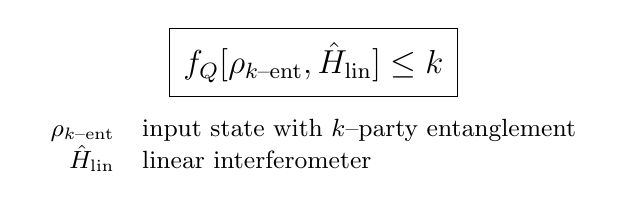
\begin{tikzpicture}
            \node[draw=black, inner sep=5pt, font=\large] (crit) at (0,0) {
                $f_Q[\rho_{k \text{--ent}}, \hat{H}_{\text{lin}}] \leq k$
            };
            \node[below=0.1cm of crit, font=\small] {
                $
                \begin{array}{rl}
                    \rho_{k \text{--ent}} & \text{input state with $k$--party entanglement} \\
                    \hat{H}_{\text{lin}} & \text{linear interferometer}
                \end{array}
                $
            };
        \end{tikzpicture}

        \column{0.45\textwidth}
        We look at the multipartite entanglement structure of symmetry protected topological phases using quantum Fisher information of non-local operators

    \end{columns}

\end{frame}

\begin{frame}{Long-range Kitaev chain}
    one-dimensional $p$-wave superconductor with \textbf{long-range coupling} $\sim 1/r^{\alpha}$

    \small
    \begin{equation*}
        H = \sum_{j} \qty[
            -t c_j^{\dagger} c_{j+1}
            -\mu \qty( c_j^{\dagger} c_j - \frac{1}{2} )
            + \frac{\Delta}{2} \sum_{r} \boxed{\frac{1}{r^{\alpha}} c_j^{\dagger} c_{j+r}}
            + \text{h.c.}
        ]
    \end{equation*}

    \begin{columns}\small
        \column{0.4\textwidth}
        \textbf{QFI of non-local spin degrees of freedom}
        \begin{itemize}\footnotesize
            \item $\sigma_j^+ = c^{\dagger}_j e^{i \pi \sum_{i < j} c_i^{\dagger} c_i} $, ~~$\sigma_j^- = e^{i \pi \sum_{i < j} c_i^{\dagger} c_i} c_j $
            \item $\hat{H}_{\text{lin}}^{\,\rho} = \sum_{j} \sigma^{\rho}_{j} $, ~$\rho=x,y$
        \end{itemize}
        We look at the scaling of $f_Q[\ket{\text{gs}}, \hat{H}_{\text{lin}}^{\,\rho}]$ with the system size $L$
        \\[10pt]
        \fbox{\parbox{\textwidth}{The scaling can be computed analytically \\ using \textbf{Toeplitz determinants}}}

        \column{0.5\textwidth}
        \input{figures/lrk-phases.tex}

    \end{columns}
\end{frame}


\begin{frame}{Bilinear-Biquadratic model}
    most general $SU(2)$--invariant isotropic spin-$1$ Hamiltonian

    \small
    \begin{equation*}
        H = J \sum_{i} \qty[
            \bm{S}_i \cdot \bm{S}_{i+1}
            - \beta \qty( \bm{S}_i \cdot \bm{S}_{i+1} )^2
        ]
        = J^{\prime}  \sum_{i} \qty[
            \cos \theta \bm{S}_i \cdot \bm{S}_{i+1}
            - \sin \theta \qty( \bm{S}_i \cdot \bm{S}_{i+1} )^2
        ]
    \end{equation*}

    \begin{columns}\small
        \column{0.35\textwidth}

        \textbf{QFI of string operators}
        \begin{itemize}\footnotesize
            \item $\widetilde{S}_j^z = \left( e^{i \pi \sum_{i < j}  S^z_i } \right) S_j^z$
            \item $\hat{O} = \sum_{j} \widetilde{S}_j^z $
        \end{itemize}
        We look at the scaling of $f_Q[\ket{\text{gs}}, \hat{O}]$ with the system size $L$


        \column{0.65\textwidth}
        \centering
        \input{figures/blbq-phases.tex}


    \end{columns}
\end{frame}
\end{document}
